\section{在实践中生成随机比特}

在密码学中,许多任务都需要随机比特,例如生成密钥和其他被称为 nonce 的短时值。在整本书中,我们假设所有参与方都能获得良好的随机源,否则许多理想的密码学目标就都不可能实现。到目前为止,我们使用 PRG 将一个短的均匀分布的秘密种子拉伸成一个长的伪随机序列。虽然 PRG 是生成伪随机比特序列的一个重要工具,但它只是故事的一部分。

在实践中,随机比特序列通常是使用\textbf{随机数生成器 (random number generator, RNG)} 生成的。RNG 和 PRG 一样输出一串随机或伪随机的比特。然而 RNG 有一个额外的接口,用于不断向 RNG 的内部状态添加熵,如图 \ref{fig:3-14} 所示。其原理是,每当系统有更多的随机熵贡献给 RNG 时,这些熵就被添加到 RNG 的内部状态中。每当有人从 RNG 中读取比特时,这些比特都是用当前的内部状态生成的。

\begin{figure}
  \centering
  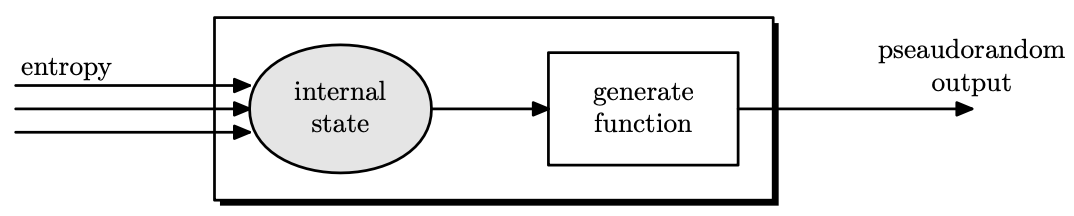
\includegraphics[width=0.7\linewidth]{figures/chapter3/fig14.png}
  \caption{一个随机数生成器}
  \label{fig:3-14}
\end{figure}

一个典型的例子是 Linux 操作系统中的 RNG,它被实现成一个名为 \texttt{/dev/random} 的设备。任何人都可以从该设备中读取到随机比特。你可以在 UNIX shell 中输出 \texttt{cat /dev/random} 来试着玩一玩这个工具,你将会看到一串无休止的、看起来很随机的字符。UNIX RNG 从一些硬件来源获得随机熵,包括:
\begin{itemize}
	\item 键盘事件:按键时间间隔能够提供随机熵;
	\item 鼠标事件:中断时间和鼠标位置都能够提供随机熵;
	\item 硬件中断:硬件中断的时间间隔也能提供较高质量的随机熵。
\end{itemize}
这些随机源能够产生连续的随机流,并会被定期异或到 RNG 的内部状态上。请注意,具体的键盘输入内容不会被用作熵的来源,通常使用的只是按键的时间,这是为了确保用户的输入内容不会通过 RNG 泄露给系统中的其他用户。

\begin{snote}[高熵的随机生成。]
上述熵源产生随机流的速度相对较慢。为了以更快的速度生成真随机比特,英特尔从 2012 年的 Ivy Bridge 处理器系列开始,增加了一个硬件随机数生成器。使用 \texttt{RdRand} 指令即可读取这个生成器的输出,它旨在提供一个快速且均匀的随机比特生成器。

为了减少生成器输出中的偏差,原始比特首先通过一个被称为``调节器"的函数,以确保在提供足够熵源作为输入时,输出是一个均匀分布的比特序列。我们在 \ref{sec:8-10} 节讨论密钥推导问题时会更详细地讨论这个问题。

\texttt{RdRand} 发生器不应该取代其他的熵源,比如上面描述的几个熵源;它只应该作为 RNG 的一个\emph{额外的}熵源来增强它们。这样一来,如果生成器有缺陷,就不会完全影响到加密应用。

英特尔的方法的一个困难是,随着时间的推移,被采样的硬件元素可能由于硬件故障而停止产生随机流。例如,被采样的比特可能总是 ``$0$",这会导致高度非随机的输出。为了防止这种情况的发生,RNG 的输出会被不断地用一套固定的统计方法来测试。如果任何一项测试报告为``非随机",发生器就会被认为有缺陷。
\end{snote}